% DO NOT COMPILE THIS FILE DIRECTLY!
% This is included by the other .tex files.

\begin{frame}[t,plain]
\titlepage
\end{frame}

\begin{frame}[t]{Topics for Today}
We will look at:

\begin{itemize}
\item Trans-dimensional MCMC
\item Nested Sampling
\end{itemize}

\end{frame}


\begin{frame}[t]{Trans-dimensional MCMC}
Trans-dimensional MCMC is useful when the model dimension is unknown. This
arises quite frequently in astrophysics.
\end{frame}


\begin{frame}[t]{Trans-dimensional examples}
Some examples from my own work: How many stars are in these images (and what are their positions and fluxes)?

\begin{center}
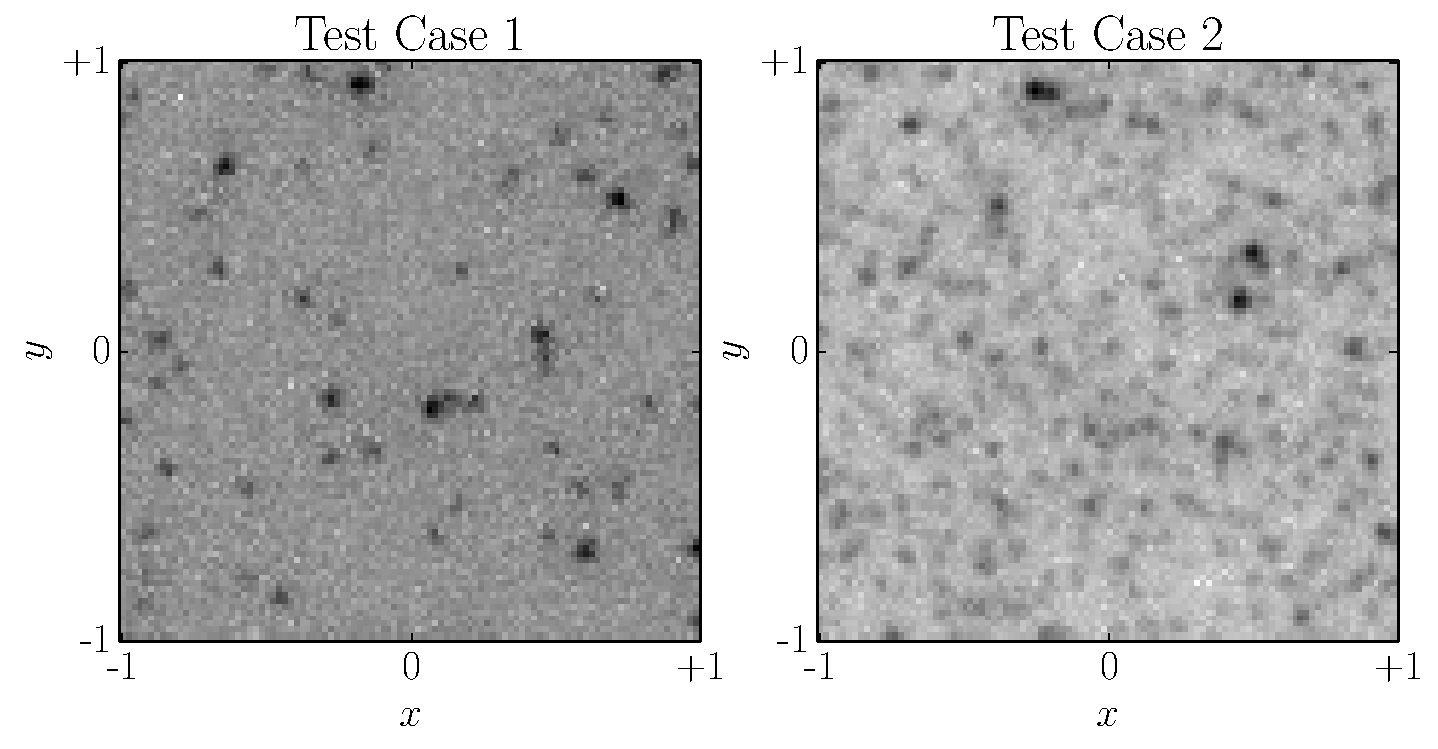
\includegraphics[scale=0.4]{starfield.pdf}
\end{center}

\end{frame}

\begin{frame}[t]{Trans-dimensional examples}
How many stars were there?

\begin{center}
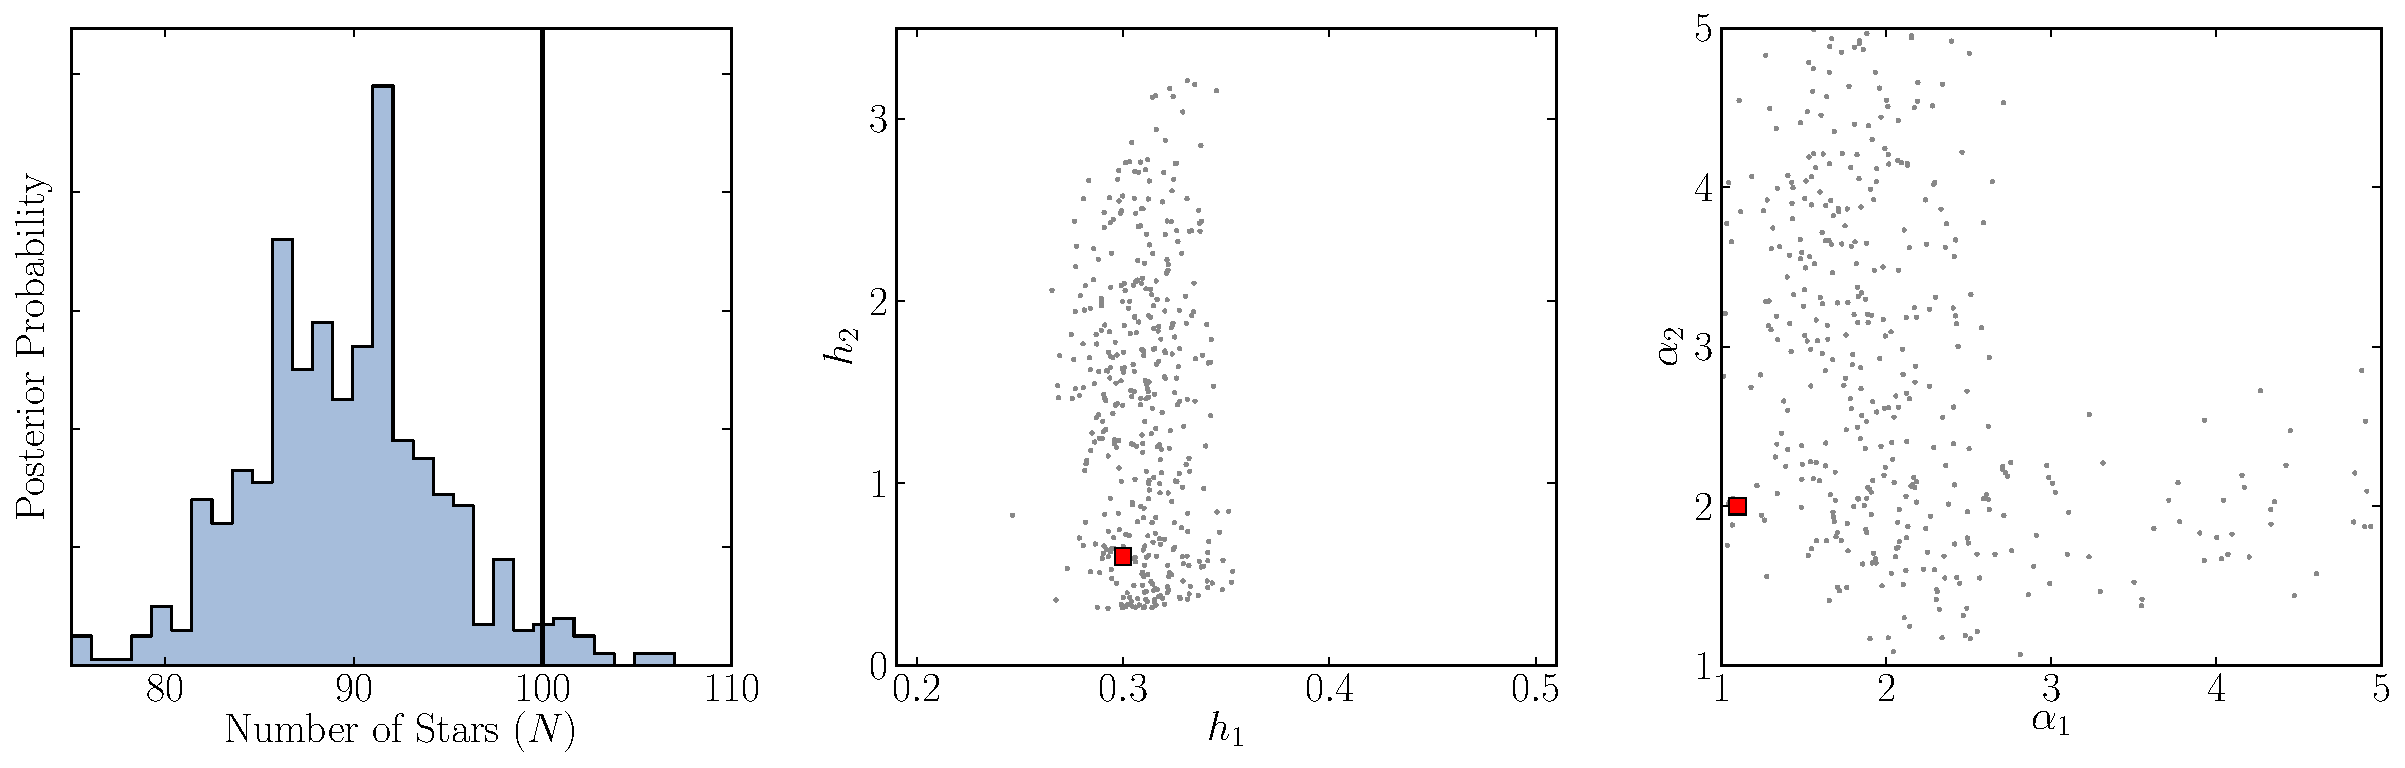
\includegraphics[scale=0.25]{inference1.pdf}
\end{center}

\end{frame}

\begin{frame}[t]{Trans-dimensional examples}
How many stars were there?
\begin{center}
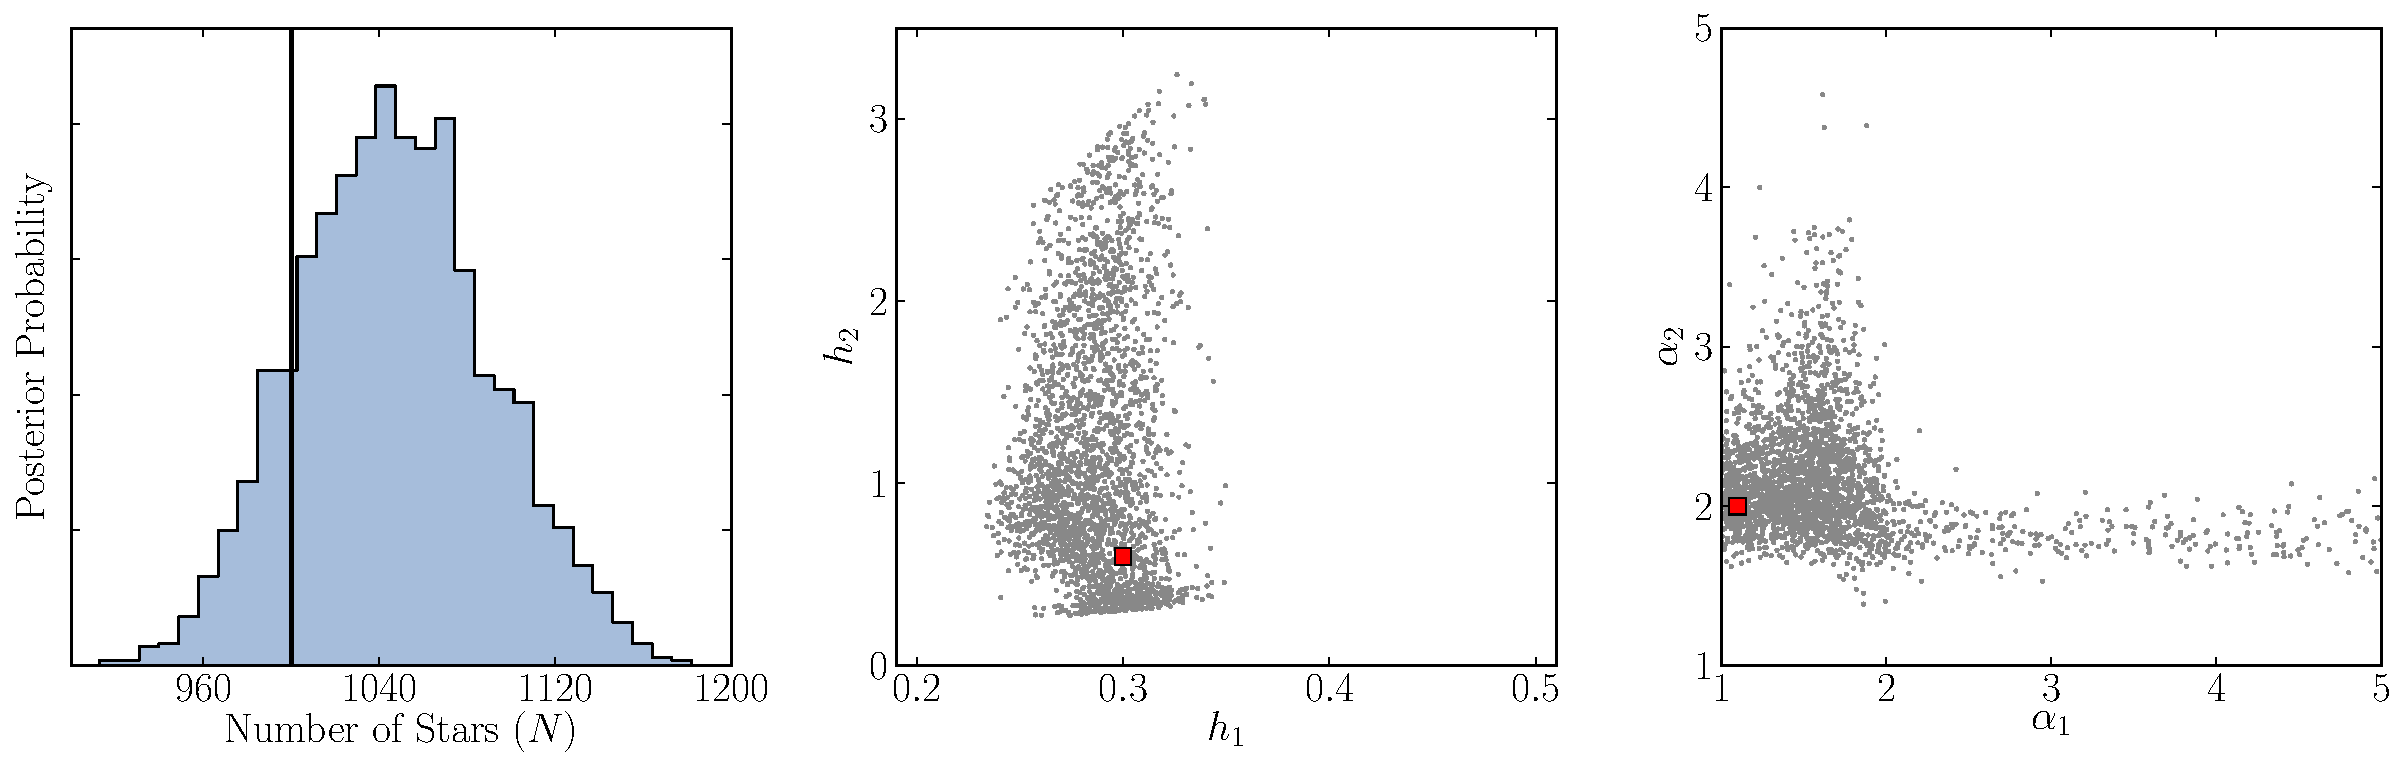
\includegraphics[scale=0.25]{inference2.pdf}
\end{center}

\end{frame}

\begin{frame}[t]{Trans-dimensional examples}
Perhaps you can see how to use MCMC to estimate the parameters of the
stars ($x$ and $y$ position, and a brightness, for each), if we knew the
number of stars.

\vspace{20pt}
But we want to know the number of stars!
\end{frame}

\begin{frame}[t]{Asteroseismology Example}

\begin{center}
\includegraphics[scale=0.4]{star.png}
Image credit: Tim Bedding
\end{center}

\end{frame}

\begin{frame}[t]{Asteroseismology: Time Series Data}

\begin{center}
\includegraphics[scale=0.22]{betahyi1.png}\\
Image credit: Tim Bedding
\end{center}

\end{frame}

\begin{frame}[t]{Asteroseismology Example: Power Spectrum}

\begin{center}
\includegraphics[scale=0.25]{betahyi2.png}\\
Image credit: Tim Bedding
\end{center}

\end{frame}

\begin{frame}[t]{Asteroseismology Example: Toy Dataset}

\begin{center}
\includegraphics[scale=0.35]{Code/asteroseismology_data.pdf}\\
\end{center}

\end{frame}


\begin{frame}[t]{Asteroseismology Example: Question}

\begin{center}
\includegraphics[scale=0.27]{Code/asteroseismology_data.pdf}
\end{center}

Given this data, how many peaks are there? And what are their parameters
(position, height, width)?

\end{frame}



\begin{frame}[t]{Asteroseismology Example}
Each of the peaks has a ``Lorentzian'' shape
(same as the Cauchy distribution!):
\begin{eqnarray}
m(x) &=& B + \sum_{i=1}^N \frac{A_i}
{\left[1 + \left(\frac{x - c_i}{w_i}\right)^2\right]} 
\end{eqnarray}

$A_i$ = amplitude of $i$th component\\
$c_i$ = center of $i$th component\\
$w_i$ = width of $ith$ component\\


\end{frame}

\begin{frame}[t]{Asteroseismology Example}
The sampling distribution/likelihood is

\begin{eqnarray*}
y_i \sim \textnormal{Exponential}(m(x_i; \theta)).
\end{eqnarray*}

i.e.
\begin{eqnarray*}
p(\{y_i\} | \theta) &=& \prod_{i=1}^n \frac{1}{m(x_i; \theta)}
\exp\left[-\frac{y_i}{m(x_i; \theta)}\right].
\end{eqnarray*}
\end{frame}


\begin{frame}[t]{Asteroseismology Example}
Some simple priors are:

\begin{eqnarray*}
N &\sim& \textnormal{Uniform}\left(\{0, 1, 2, ..., 9, 10\}\right)\\
\log(B) &\sim& \textnormal{Uniform}\left[\log(10^{-3}, \log(10^{3})\right]\\
x_i &\sim& \textnormal{Uniform}\left(x_{\rm min}, x_{\rm max}\right)\\
A_i &\sim& \textnormal{Exponential}(\textnormal{mean=10})\\
\log(w_i) &\sim& \textnormal{Uniform}\left[\log(0.01 x_{\rm range}), \log(x_{\rm range})\right]
\end{eqnarray*}

\end{frame}



\begin{frame}[t]{Recall: Monte Carlo}
\begin{columns}[T]
\begin{column}{0.35\textwidth}
  \vspace{20pt}
  \begin{itemize}
  \setlength{\itemsep}{10pt}
  \item {\bf Marginalisation} becomes trivial
  \item We can quantify all uncertainties we might be interested in
  \end{itemize}
\end{column}
\hfill
\begin{column}{0.5\textwidth}
  \hspace{-30pt}
  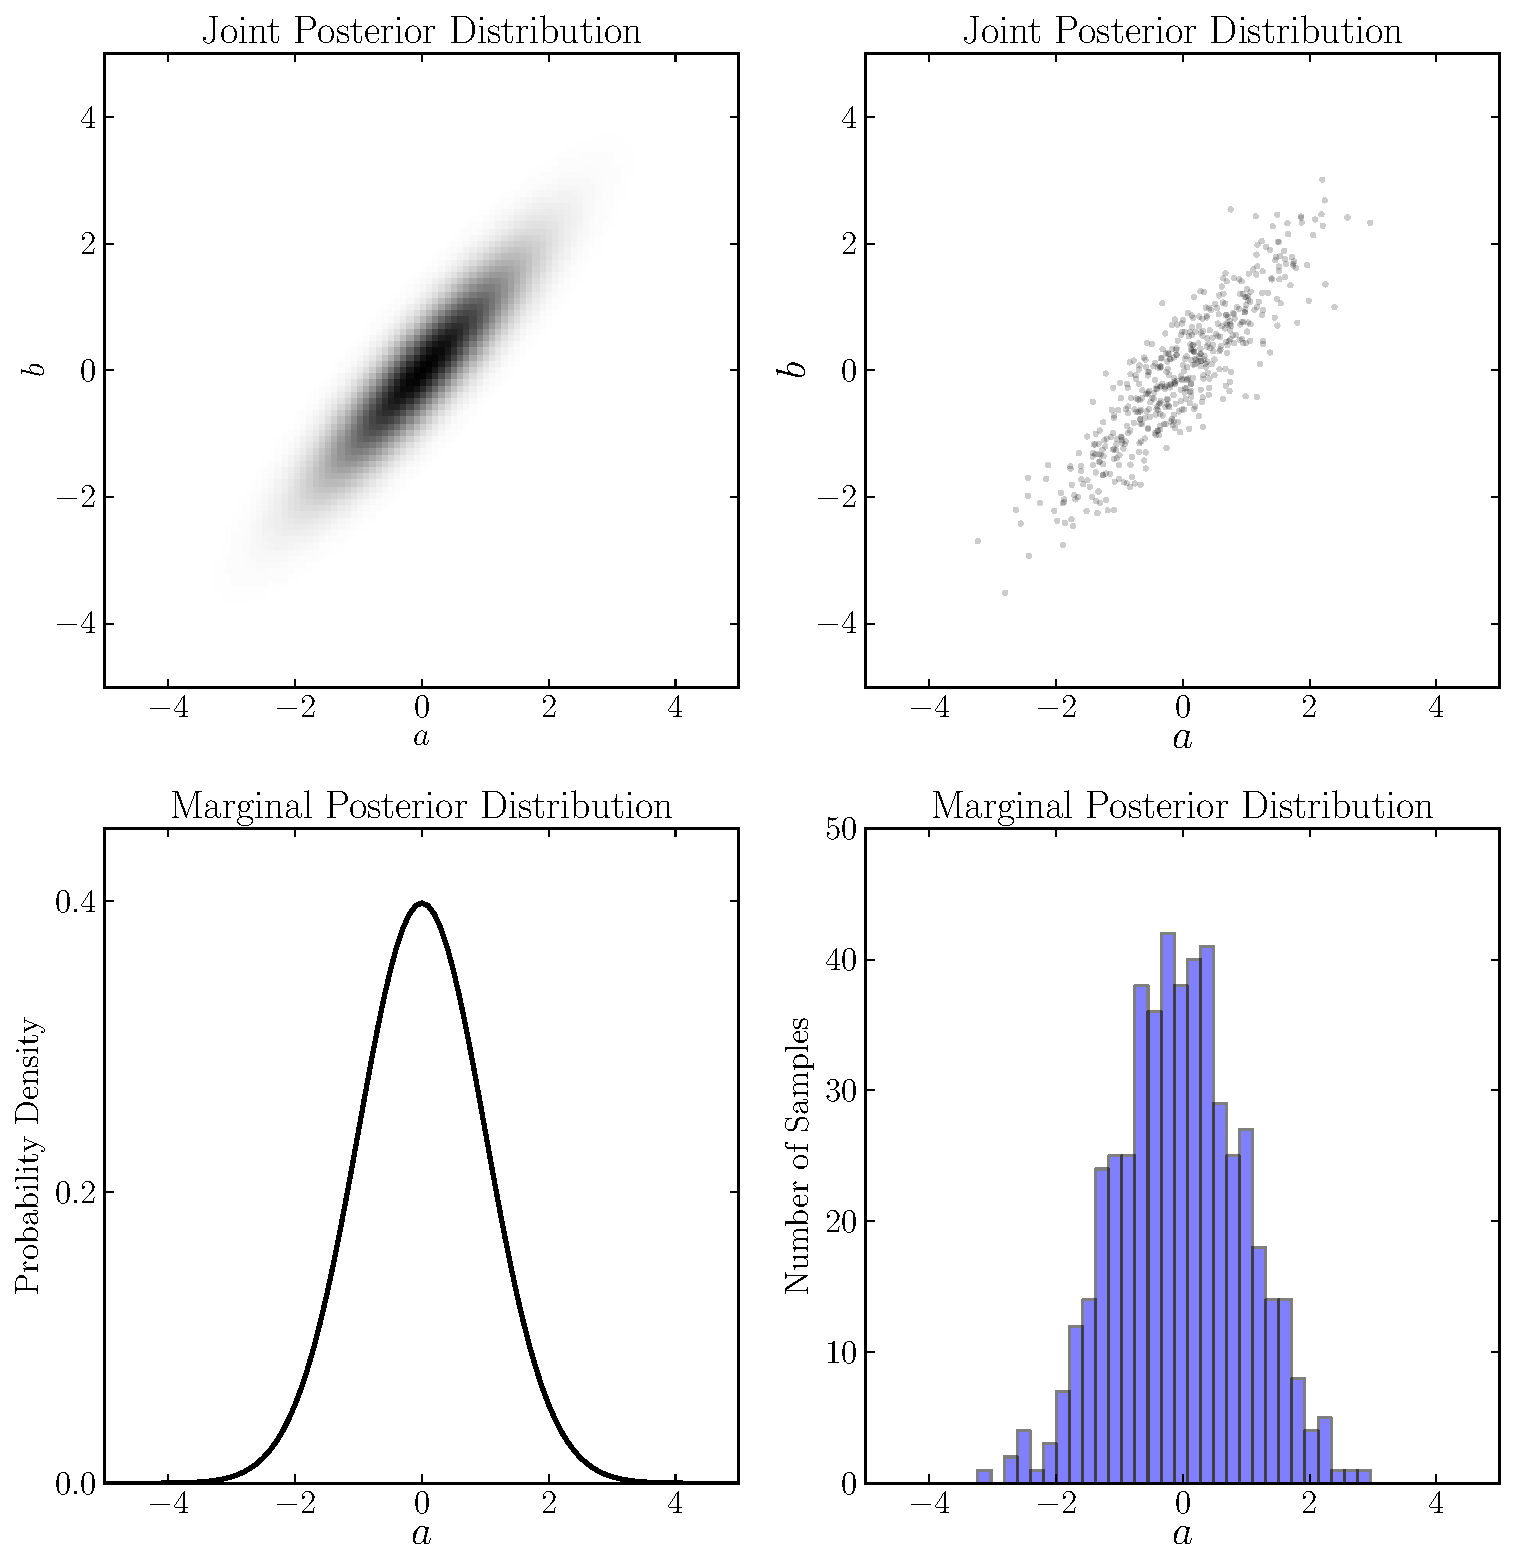
\includegraphics[scale=0.22]{marginalisation.pdf}
\end{column}

\end{columns}
\end{frame}


\begin{frame}[t]{Recall: The Metropolis Algorithm}

\begin{itemize}
\item Start at some point $\theta$ in the hypothesis space.
\item Loop\\
$\{$
  \begin{itemize}
  \item Generate {\bf proposal} from some distribution $q(\theta' | \theta)$
  (e.g. slightly perturb the current position).
  \item With probability $\alpha = \min\left(1, \frac{p(\theta')p(D|\theta')}{p(\theta)p(D|\theta)}\right)$, accept the proposal (i.e. replace $\theta$ with $\theta'$).
  \item Otherwise, stay in the same place.
  \end{itemize}
$\}$
\end{itemize}
\end{frame}


\begin{frame}[t]{Trans-Dimensional MCMC}
For problems of unknown dimensionality, the hypothesis space is the union
of several fixed-dimension hypothesis spaces. To do MCMC with these models,
you need a way to move between models with different numbers of components.

\begin{center}
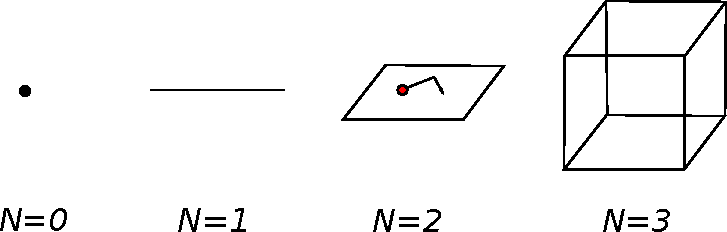
\includegraphics[scale=0.7]{drawing.pdf}
\end{center}

\end{frame}


\begin{frame}[t]{Approaches to Trans-Dimensional MCMC}
There are several approaches:

\begin{itemize}
\item Reversible Jump MCMC (Green, 1995)\\
\item Birth and Death MCMC (Stephens, 2000)
\end{itemize}

\end{frame}


\begin{frame}[t]{Approaches to Trans-Dimensional MCMC}
We will do our MCMC like this:

\begin{itemize}
\item Put 10 components in the model, and do MCMC as usual.
\item Interpret the parameter $N$ as the {\bf number of components that are ``switched on''}
\end{itemize}

\end{frame}


\begin{frame}[t]{Code for the priors}
Let's take a look at the Python code for the priors. Remember, the prior
appears in two places:

\begin{itemize}
\item The function {\tt from\_prior}, which we use to generate a starting point
\item The function {\tt log\_prior}, which calculates the log of the prior
density, which is used to determine the acceptance probability.
\end{itemize}
\end{frame}


\begin{frame}[t]{Code for the likelihood}
Let's take a look at the Python code for the likelihood function.\\

\vspace{20pt}

Note how the calculation of the model curve $m(x)$ only sums over the first
$N$ model components, the ones that are {\bf switched on}.

\end{frame}

\begin{frame}[t]{Label Switching Degeneracy}
Imagine we found a solution with two peaks like this:

\begin{eqnarray*}
\textnormal{Peak 1}: \{A, t_c, w\} &=& \{5, 3, 2\}\\
\textnormal{Peak 2}: \{A, t_c, w\} &=& \{3, 7, 1\}
\end{eqnarray*}

Then the following solution is completely equivalent:
\begin{eqnarray*}
\textnormal{Peak 1}: \{A, t_c, w\} &=& \{3, 7, 1\}\\
\textnormal{Peak 2}: \{A, t_c, w\} &=& \{5, 3, 2\}
\end{eqnarray*}

\end{frame}

\begin{frame}[t]{Label Switching Degeneracy}
When there are $N$ peaks, the posterior will have $N!$ identical modes,
corresponding to switching the order of the peaks.\\

\vspace{20pt}
We can add a proposal move that switches labels. Since the meaning of the
models is the unchanged, this proposal will always be accepted. 
\end{frame}


\begin{frame}[t]{Label Switching Degeneracy}
The {\tt shuffle} function chooses two switched-on peaks ``at random''
and swaps their parameter values.
\end{frame}



\begin{frame}[t]{Part II: Nested Sampling}
Nested Sampling is a Monte Carlo method (not necessarily MCMC) that was
introduced by John Skilling in 2004.

It is very popular in astrophysics and has some unique strengths.
\end{frame}


\begin{frame}[t]{Marginal Likelihood}
The {\bf marginal likelihood} is useful for ``model selection''. Consider
two models: $M_1$ with parameters $\theta_1$, $M_2$ with parameters $\theta_2$.
The marginal likelihoods are:
\begin{eqnarray*}
p(D | M_1) &=& \int p(\theta_1 | M_1) p(D | \theta_1, M_1) \, d\theta_1\\
p(D | M_2) &=& \int p(\theta_2 | M_2) p(D | \theta_2, M_2) \, d\theta_2
\end{eqnarray*}

These are the normalising constants of the posteriors, within each model.
\end{frame}



\begin{frame}[t]{Bayesian Model Selection}
If you have the marginal likelihoods, it's easy:

\begin{eqnarray*}
\frac{P(M_1 | D)}{P(M_2 | D)} &=& \frac{P(M_1)}{P(M_2)}
\times \frac{P(D | M_1)}{P(D | M_2)}.
\end{eqnarray*}
\end{frame}


\begin{frame}[t]{Challenging features}
Another motivation: standard MCMC methods can get stuck in the following
situations:
\begin{center}
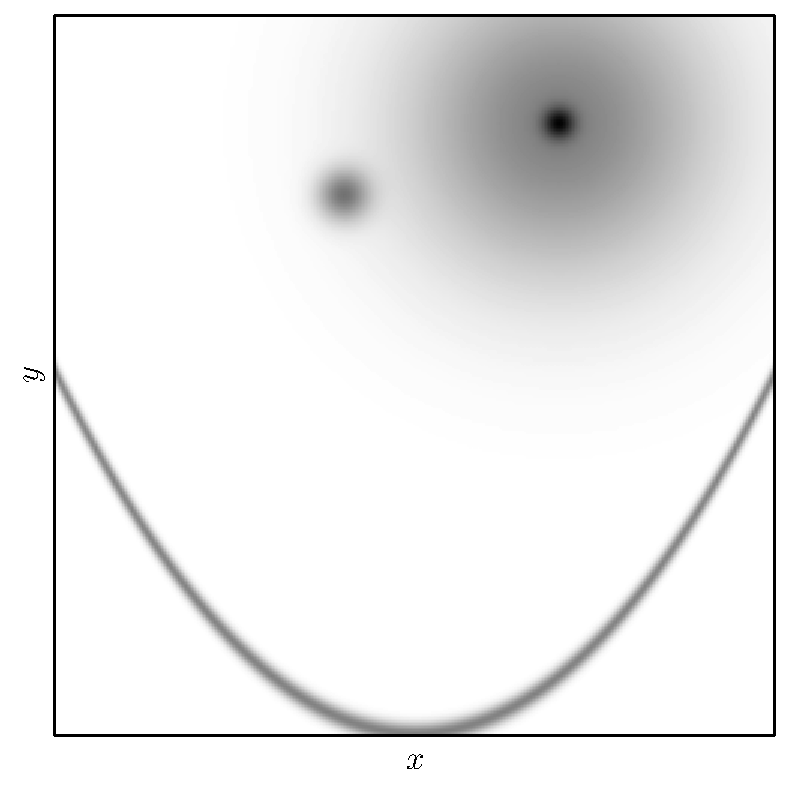
\includegraphics[scale=0.4]{challenges.pdf}
\end{center}
\end{frame}

\begin{frame}{\small{\textbf{Nested Sampling}}}
Nested Sampling was built to estimate the marginal likelihood.

But it can also be used to generate posterior samples, and it can potentially
work on harder problems where standard MCMC methods get stuck.
\end{frame}

\begin{frame}[t]{Nested Sampling}
The key idea of Nested Sampling: 

\begin{figure}
\begin{center}
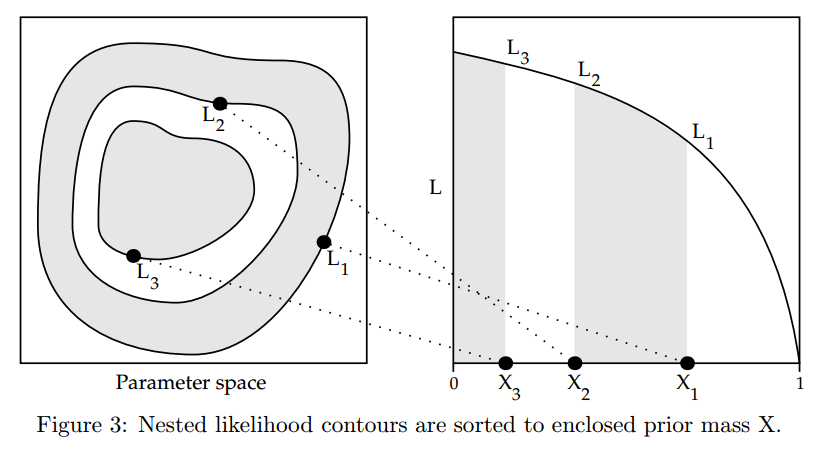
\includegraphics[scale=0.4]{ns.png}
\end{center}
\end{figure}


\end{frame}

%##########################################################################################################################################

%%##########################################################################################################################################
%\begin{frame}{\small{\textbf{Nested Sampling}}}
%Other methods to estimate the evidence:\\~\\
%\begin{itemize}
%\item [*] Harmonic mean.
%\item [*] Thermodynamic integration.
%\item [*] Steppingstone sampling.
%\end{itemize}
%\end{frame}
%#########################
%%##########################################################################################################################################
%\begin{frame}{\small{\textbf{Nested Sampling}}}
%Consider the \textbf<1,2>{positive} random variable $X$ with probability density function $f(x)$ and distribution function $F(x)$. So

%\begin{align*}
%\text{E}(X) = \int_{0}^{\infty} x f(x) \text{d}x \visible<2>{ \equiv \int_{0}^{\infty} (1- F(x))\text{d}x	}
%\end{align*}

%\end{frame}
%%##########################################################################################################################################
%\begin{frame}{\small{\textbf{Nested Sampling}}}
%\begin{overprint}
%\onslide<1>
%\begin{figure}[]    		
%		\includegraphics[scale=0.28,clip=true,angle=0]{Patricio/CDF1.pdf}
%		\caption{Distribution function for a positive random variable X.}
%\end{figure}
%\onslide<2>
%\begin{figure}[]    		
%		\includegraphics[scale=0.28,clip=true,angle=0]{Patricio/CDF2.pdf}
%		\caption{Distribution function for a positive random variable X.}
%\end{figure}
%\end{overprint}
%\end{frame}
%%##########################################################################################################################################
%\begin{frame}{\small{\textbf{Nested Sampling}}}
%Note that $L(\bm\theta | \bm Y ) > 0$ can be seen as a positive random variable with $\bm \theta \sim \pi(\bm\theta)$
%\visible<2,3>{
%\begin{align*}
%\Longrightarrow Z  = \idotsint \pi(\bm\theta) L(\bm{\theta}|\bm{Y}) \text{d}\bm{\theta} = \text{E}_{\pi}\big(L(\bm{\theta}|\bm{Y})\big) 
%\end{align*}}
%\visible<3>{
%\begin{align*}
% = \int_{0}^{\infty} (1-F(\lambda))\text{d}\lambda
%\end{align*}
%where $\lambda = L(\bm{\theta}|\bm{Y})$ and
%\begin{align*}
%F(\lambda) = \idotsint \limits_{L (\bm{\theta})< \lambda} \pi(\bm\theta) \text{d}\bm\theta
%\end{align*}}
%\end{frame}
%##########################################################################################################################################
\begin{frame}{\small{\textbf{Nested Sampling}}}
Define
\begin{align*}
	X(l) = \int \pi(\theta) \mathds{1}\left(L(\theta) > l\right)d^\theta
\end{align*}

$X$ is the {\bf amount of prior probability} with likelihood greater than $l$.
\end{frame}
%##########################################################################################################################################
\begin{frame}{\small{\textbf{Nested Sampling}}}
\begin{overprint}
\onslide<1>
	\begin{figure}
		\includegraphics[scale=0.28,clip=true,angle=0]{Patricio/AreaZ.pdf}
	\caption{Likelihood function with area Z.}
	\end{figure}
	$\mathcal L (0.95) = 0.001$ means that 95\% of the draws $\bm\theta$ from the prior distribution $\pi(\bm\theta)$ will have likelihoods greater than 0.001.		
\onslide<2>
\begin{figure}
	\includegraphics[scale=0.28,clip=true,angle=0]{Patricio/Posterior.pdf}
	\caption{Posterior sample.}
\end{figure}	
\end{overprint}
\end{frame}
%##########################################################################################################################################
\begin{frame}{\small{\textbf{Nested Sampling}}}
This area could be approximated by standard quadrature (numerical integration) method 
\begin{align*}
\widehat{Z} = \sum_{i=1}^{k}(\xi_{i-1}-\xi_{i}) \mathcal L_{i}
\end{align*}
where $\mathcal L_{i}= \mathcal L (\xi_{i})$ and $0<\xi_k<\cdots<\xi_{1}<\xi_{0}=1$.
\end{frame}
%######################################%##########################################################################################################################################
\begin{frame}{\small{\textbf{Nested Sampling}}}
Calculating $\mathcal L_{i}$ values. \\~\\

\begin{itemize}
	\item [*] Sample $\bm\theta=\{\theta_{1}, \ldots , \theta_{N}\}$ from the prior $\pi(\theta)$.
	\item [*] \visible<2,3,4,5>{Set $\mathcal L_{i} = \text{min}\{L(\theta_1), \ldots , L(\theta_N)\} = L(\theta_{j})$.}
	\item [*] \visible<3,4,5>{Replace $\theta_{j}$ by a $\theta$ draw from $\pi(\theta)$ conditional upon $L(\theta)>L(\theta_{j})$.}
\end{itemize}

\visible<4,5>{Repeat for as long as needed.}\\~\\

\visible<5>{The points replaced generate a sequence of \textit{discarded points}.}
\end{frame}
%##########################################################################################################################################
\begin{frame}{\small{\textbf{Nested Sampling}}}
\begin{overprint}
\onslide<1>
\begin{figure}[]    		
		\includegraphics[scale=0.28,clip=true,angle=0]{Patricio/SampleLike.pdf}
		%\caption{}
\end{figure}
\onslide<2>
\begin{figure}[]    		
		\includegraphics[scale=0.28,clip=true,angle=0]{Patricio/SampleLike1.pdf}
		\caption{The $\mathcal L$ values }
\end{figure}
\onslide<3>
\begin{figure}[]    		
		\includegraphics[scale=0.28,clip=true,angle=0]{Patricio/SampleLike2.pdf}
		\caption{Relationship between $\mathcal L$ and $\xi$ values.}
\end{figure}
\end{overprint}
\end{frame}
%##########################################################################################################################################
\begin{frame}{\small{\textbf{Nested Sampling}}}
\begin{columns}[T]\column{0.6\textwidth}
Estimating $\xi_{i}$ values.\\~\\
Consider the decreasing sequence
\begin{align*}
0<\xi_{N}<\cdots<\xi_{1}<\xi_{0}=1
\end{align*}
where $\xi_{j}\sim\text{Uniform}(0,1)$, for $j=1,\ldots,N,$ \visible<2,3,4,5,6>{which implies that 
\begin{align*}
t = \text{max}\{ \xi_1,\ldots,\xi_{N}\} \sim \text{Beta}(N,1)
\end{align*}
}
\visible<3,4,5,6>{So, we could set
\begin{align*}
\xi_{1}=t_{1},\quad \xi_{2}=t_{1}t_{2},\quad \ldots \quad,\quad \xi_{i}=\prod_{j=1}^{i}t_{j}, \ldots
\end{align*}} 
\visible<4,5,6>{or alternatively, we will consider that}
\column{0.4\textwidth}
\begin{figure}
 %\hspace{4cm}  \vspace{0.001cm}
   \includegraphics[width=1.1\textwidth,natwidth=69,natheight=87]{Patricio/xis.pdf}
\end{figure}
\end{columns}
\begin{align*}
\visible<4,5,6>{\text{E}(\log t) = -\frac{1}{N}} 
\visible<5,6>{\Rightarrow \text{If we set}\quad \log t = -\frac{1}{N}}&\visible<5,6>{\Rightarrow t = e^{-1/N}}\\
&\visible<6>{\Rightarrow \xi_{i}= e^{-i/N}}
\end{align*}
\end{frame}
%##########################################################################################################################################
\begin{frame}{\small{\textbf{Nested Sampling}}}
\begin{figure}[]    		
		\includegraphics[scale=0.28,clip=true,angle=0]{Patricio/PriorExplore.pdf}
		\caption{Discrete sequence of $\xi$ values.}
\end{figure}
\end{frame}
%##########################################################################################################################################
%\begin{frame}{\small{\textbf{Nested Sampling}}}
%Nested Sampling is given by the following steps:
%\begin{enumerate}
%\item Sample $N$ points $\theta_1, \ldots ,\theta_N$ from the prior;
%\item Initialize $Z=0$ and $X_0=1$;
%\item Repeat for $i=1, \ldots, j$;
%			\begin{description}
%				\item[i)  ] find the lowest likelihood $L_i=L(\theta_{l})$;
%				\item[ii) ] set $X_i=\exp(-i/N)$;
%				\item[iii)] set $w_i= X_{i-1}-X_{i}$;
%				\item[iv)] update $Z= w_{i}L_{i} + Z$; and				
%				\item[v)  ] replace $\theta_l$ by drawing a new point $\theta$ from the prior distribution restricted to $L(\theta)>L_i$.
%			\end{description}
%\end{enumerate}
%\end{frame}
%###########%##########################################################################################################################################
\begin{frame}{\small{\textbf{Posterior Sample}}}
The Posterior sample can be obtained by drawing from the discarded points $\theta_1,\theta_2,\theta_3 \ldots$ with the following weights
\begin{align*}
p_{j} = \frac{L_{j} w_{j}}{Z} 
\end{align*}
where $w_{j}=\xi_{j-1} - \xi_{j}$.
\\~\\
\visible<2>{
The maximum number of representative posterior samples is given by

\begin{align*}
\mathcal N = \exp \Bigg( - \sum_{j=1}^{m} p_j \log p_j \Bigg)
\end{align*}
}
\end{frame}


